\documentclass{article}

\usepackage[utf8]{inputenc}
\usepackage{setspace}
\usepackage{geometry}
\usepackage{graphicx}
\usepackage{caption}
\usepackage{indentfirst}
\usepackage{anyfontsize}
\usepackage{textcomp}
\usepackage{amsmath}
\usepackage{float}
\usepackage{changepage}
\usepackage [english]{babel}
\usepackage [autostyle, english = american]{csquotes}
\MakeOuterQuote{"}

\graphicspath{}



\title{Diabetes Modeling}
\author{Geneva Porter \textbf{816408535}}
\date{09 November 2018}

%\begin{figure}[H]
%\centering{\includegraphics[width=10cm]{FILENAME.eps}}
%	\caption*{\textbf{CAPTION}}
%\end{figure}

%$\begin{bmatrix}
%11      & 12  \\
%21      & 22  \\
%\end{bmatrix}$

\begin{document}
	
\begin{titlepage}
\maketitle
\thispagestyle{empty}


\begin{center}
	
\large \it San Diego State University 
	
Professor Mahaffy, Math 636

\end{center}
\end{titlepage}


\section*{Problem 1}

In this problem, we are introduced to a model measuring glucose levels in the blood of diabetic patients. This model is described by the equation $G(t)$, given by:

\begin{center}
	$G(t) = G_0+Ae^{-\alpha t}cos(\omega(t-\delta))$
\end{center}

Where $G_0$, $A$, $\alpha$, $\omega$, and $\delta$ are parameters to be determined by fitting the model to data for individual patients. Figure 1 (below) shows the data and fitted model for both patients. This model has significant strengths, as the sinusoidal curve in the model allows an accurate prediction of a patient's cyclical rise and fall in blood sugar, while the negative exponential term ensures the rapid dampening in blood sugar levels consistent with metabolic process. One weakness of this model is that it needs 5 parameters in order to be fitted to an individual, which adds complexity and higher computational cost. It also does not account for the dangerous long term drop in blood sugar that a diabetic patient sees with prolonged fasting. Below we discuss the two curves and how the parameters of the model for each patient act as a diagnosis tool.


\begin{figure}[H]
\centerline{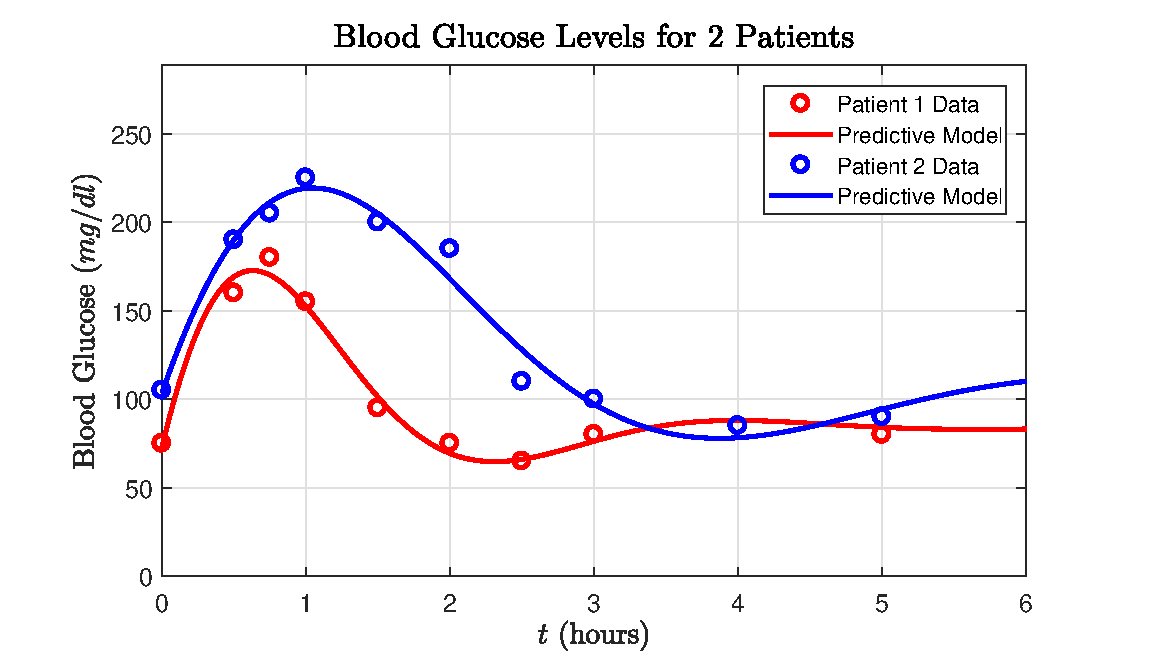
\includegraphics[width=16cm]{f1.eps}}
	\caption*{\textbf{Figure 1}}
\end{figure}

\pagebreak

\subsection*{Patient 1}

The data for patient 1 shows a steep initial rise in blood sugar in the first 45 minutes, with a gradual decline in blood sugar for the next hour. The patient's blood sugar stays around 80 mg/dl after 2 hours, which is consistent with the initial fasting level. This behavior generally indicates that patient 1 is not diabetic. If we apply the Oral Glucose Tolerance Test (OGTT) to patient 1, then he or she qualifies as normal for $t=0$, $t=1$, and $t=2$, because the blood sugar level is below 110, 180, and 140 mg/dl at those times, respectively. In addition, the parameters for this patient's data yield a $T_0$ measurement of $2\pi/\omega_0\approx3$, which is below the minimum value of 4 achieved by diabetic patients. For these three reasons, it is safe to say that this patient is not diabetic.

\vspace{2mm}

The model for patient 1, shown in red, is a very good fit for the data, with a sum of squared errors of $\approx303$. We can see that the data has little deviance from the model curve. However, one data point is a little off. The data indicates the patient achieved a blood sugar level above the maximum predicted by the model, but only by about 10 mg/dl. Otherwise, we can consider this model a good predicative tool for patient 1.

\subsection*{Patient 2}

Figure 2 (below) shows the data and model for patient 2. Like patient 1, the data shows a steep initial rise in blood sugar. However, patient 2's blodd sugar rises for the first hour, and does not level off to fasting level until hour 3. This behavior generally indicates that patient 2 may be diabetic. The OGTT confirms this generalization. Even though patient 1's fasting blood sugar at $t=0$ is below the diabetic threshold by 5 mg/dl, the criteria for $t=1$ and $t=2$ is satisfied, with levels above 180 and 140 mg/dl, respectively. In addition, the parameters for this patient's data yield a $T_0$ measurement of $2\pi/\omega_0\approx5$, which is above the minimum value achieved by diabetic patients. For these three reasons, it is safe to say that this patient has a positive diagnosis of diabetes.

\vspace{2mm}

The model for patient 2 is an ok fit for the data, with a sum of squared errors of $\approx780$. There is slightly more deviance from the curve than seen in the model for patient 1, largely due to the two data points at $t=2$ and $t=2.5$. During this time, the patient's blood sugar drops more dramatically than the model predicts. The model also had a higher amplitude cycle after $t=3$ that is not consistent with the data. While this model may fit a non-diabetic patient well, it is not as good of a fit for a diabetic patient.

\pagebreak

\section*{Problem 2}

In this problem, we will examine the model introduced by the 2007 SIAM article  "Modeling Cyclic Waves of Circulating T Cells in Autoimmune Diabetes" by J Mahaffy and L Edelstein-Keshet. It examines the phenomena behind the cyclical fluctuation of the T-cells responsible for killing insulin-secreting $\beta$ cells, which lead up to the onset of diabetes. The article offers a mathematical model that suggests immunity response regulates this cycle. Studies on non-obese diabetic (NOD) mice were referenced to formulate this model. We will be examining a reduced version of the model, given by:

\begin{center}
	$\dfrac{dA}{dt}=(\sigma+\alpha_1M)f_1(p)-(\beta+\delta_A)A-\epsilon A^2$
\end{center}

\begin{center}
	$\dfrac{dM}{dt}=\beta2^{m_1}f_2(p)A-f_1(p)\alpha_2M-\delta_MM\hspace{3mm}$
\end{center}

\begin{center}
	$\dfrac{dE}{dt}=\beta2^{m_2}(1-f_2(p))A-\delta_EE\hspace{15mm}$
\end{center}

\begin{center}
	with $p\approx(RB/\delta_p)E$, $f_1(p)=\dfrac{p^n}{k_1^n+p^n}$, and $f_2(p)=\dfrac{ak_2^m}{k_2^m+p^m}$
\end{center}

For this exercise, all the parameters are given. $A(t)$ is the population of activated T-cells, $M(t)$ is the population of memory T-cells, and $E(t)$ is the population of effector T-cells at time $t$. Also, $f_1(p)$ and $f_2(p)$ are peptide-dependent functions, with $p(t)$ being the peptide level. The population of $\beta$ cells remains a constant. We will examine 2 models using this system by setting $\delta_p$, the peptide turnover rate, to either 1 or 1.5. For this simplified model, we will examine the behavior of the $A$, $M$, and $E$ cells given a constant $\beta$ cell population. For each model, 3 positive equilibria were found.

\subsection*{Model for $\delta_p=1$}

Figure 2 shows time series graphs for the model with parameter $\delta_p=1$. Values near the 3 equilibria were examined. The first equilibrium ($e_1$) at (0,0,0) is the disease free state, representing NOD mice that do not have diabetes. This equilibrium is stable with all negative eigenvalues of -1, -0.3, and -0.01. Setting the initial conditions to $e_1+\Delta$, with $\Delta=0.001$, resulted in each function returning to the (0,0,0) state. We can see that $A(t)$ and $E(t)$ returned to 0 in about 5 and 15 days, respectively. $M(t)$ is trending downward and eventually returns to zero after several hundred days. The stability of this equilibrium guarantees that small perturbations will collapse each function to zero, as in non-diabetic subjects. 

\vspace{2mm}

The second graph in figure 2 shows a positive perturbation from the second equilibrium, $e_2$, at $\approx$(0.13, 0.01, 0.04). This equilibria is a saddle point. It has a single stable manifold with a negative eigenvalue of -2.4 and a 2-dimensional unstable manifold with complex eigenvalues $\approx0.009\pm0.57i$. $A(t)$, $M(t)$ and $E(t)$ first oscillate about the equilibrium, but degrade to a cycle that resembles a disease state after several hundred days. Since this equilibrium is unstable, this behavior is expected.


\pagebreak

The third graph in Figure 2 models positively diagnosed NOD mice. A perturbation of $+\Delta$ was made from the equilibrium $e_3$. This equilibrium is a saddle point at $\approx$(0.02, 0.13, 0.001). It has a 2-dimensional stable manifold and one unstable manifold, with two negative eigenvalues at approximately -1.53 and -0.019 and one positive eigenvalue at about 0.210. After the initial T-cell attack, shown by a sharp increase and decreases of activated cells, the model continues into cyclical behavior. If we examine the peak of the first cycle, activated T-cell count increases corresponding with memory cells increasing just before and effector cells increasing just after. This memory-activated-effector cycle is consistent with the disease model presented in the paper. However, this model shows long-term cyclical behavior rather than the short-term behavior of the onset of diabetes. This is due to the lack of beta cell change feedback, so this model is primarily useful for examining the early stages of diabetes, before the $\beta$ cells are depleted.


\subsection*{Model for $\delta_p=1.5$}

Figure 3 shows time series graphs for the model with parameter $\delta_p=1.5$, and has many similarities with the $\delta_p=1$ model. Values near the 3 equilibria were examined. The first equilibrium ($e_1$) at (0,0,0) is the disease free state. Identical to the previous discussion, This equilibrium is stable with all negative eigenvalues at -1, -0.3, and -0.01. Setting the initial conditions to $e_1+\Delta$ resulted in each function returning to the (0,0,0) state as expected. This graph is visually identical to the one for $\delta_p=1$, and indicates that small perturbations will collapse each function to zero as well. 

\vspace{2mm}

The second graph in figure 2 shows a positive perturbation from the second equilibrium $e_2$ at $\approx$(0.18, 0.02, 0.05). Like the last model, $e_2$ is also a saddle point. It has a single stable manifold with a negative eigenvalue of -2.5 and a 2-dimensional unstable manifold with complex eigenvalues at $\approx$$0.010\pm0.57i$. This graph also achieves a cyclical pattern, but significantly sooner than its $\delta_p=1$ counterpart. 

\vspace{2mm}

The third graph in Figure 3 models positively diagnosed NOD mice. Again, a perturbation of $+\Delta$ was made from the equilibrium $e_3$. This equilibrium is a saddle point at $\approx$(0.02, 1.70, 0.002). It has a 2-dimensional stable manifold and one unstable manifold, with two negative eigenvalues around -1.55 and -0.019 and one positive eigenvalue at about 0.208. It is very similar to the previous model for $\delta_p=1$, however its first peak has a slightly higher amplitude. This may indicate that a NOD mouse with T-cells exhibiting this behavior at a given beta level will develop diabetes more quickly. 




\begin{figure}[H]
	\centering{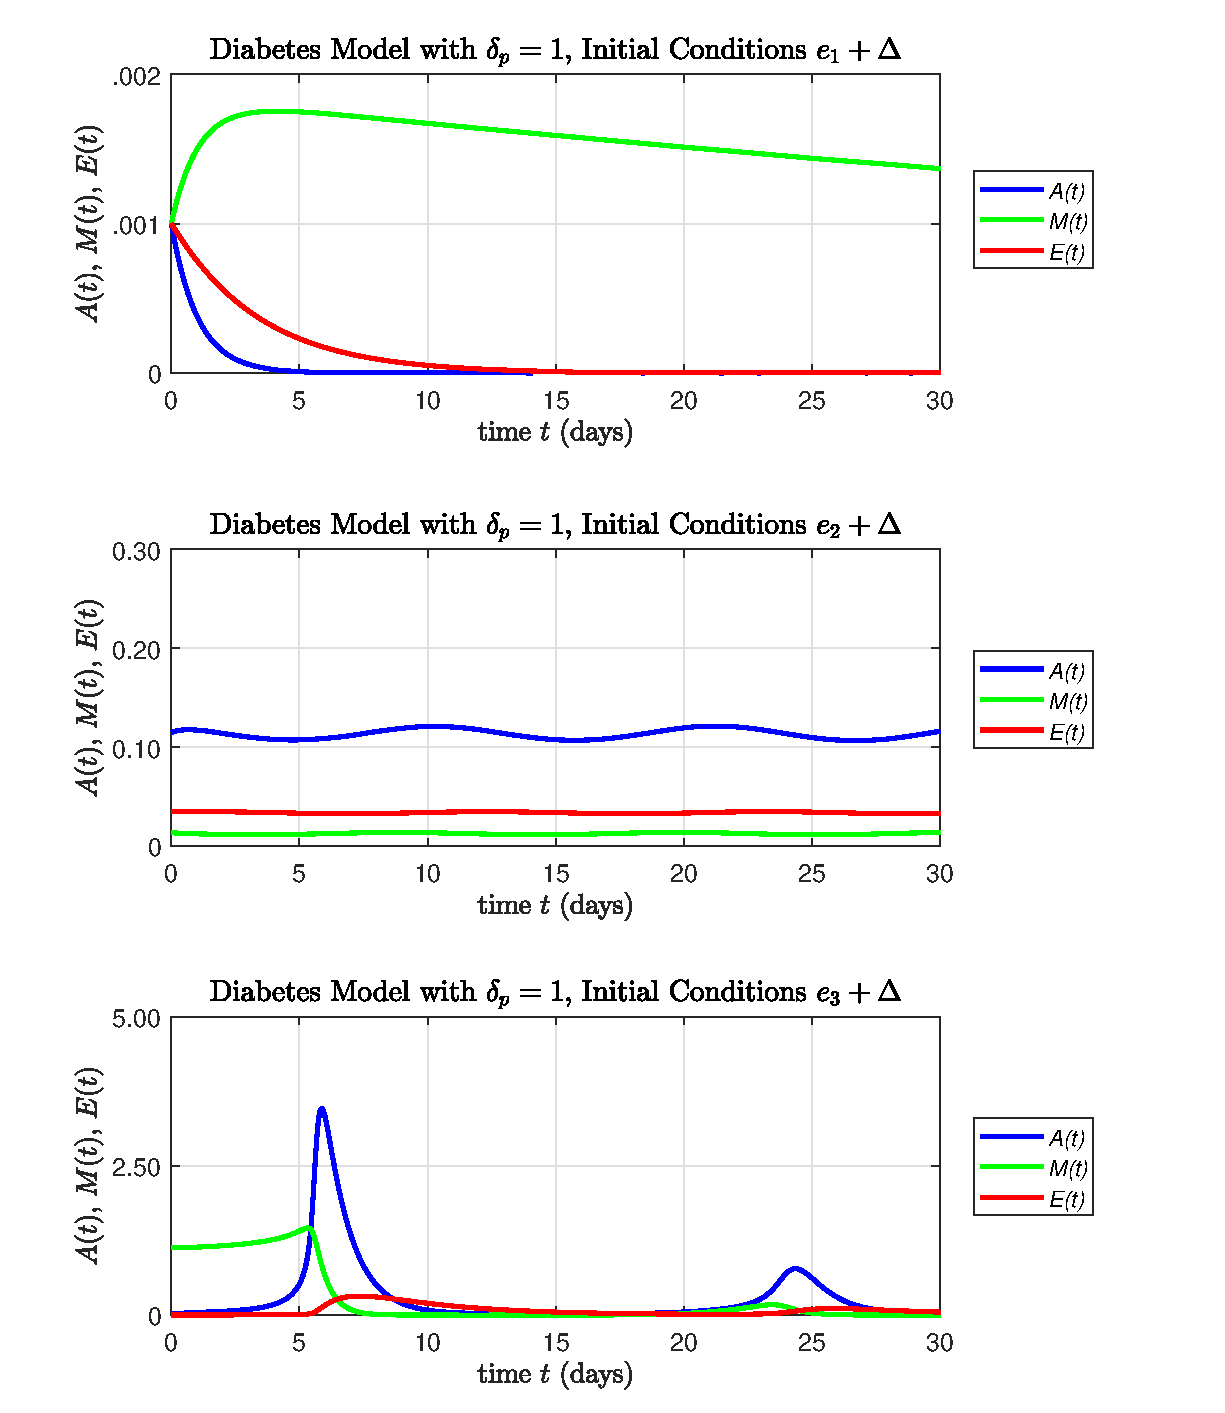
\includegraphics[width=16cm]{f2_3.eps}}
	\caption*{\textbf{Figure 2}}
\end{figure}

\begin{figure}[H]
	\centering{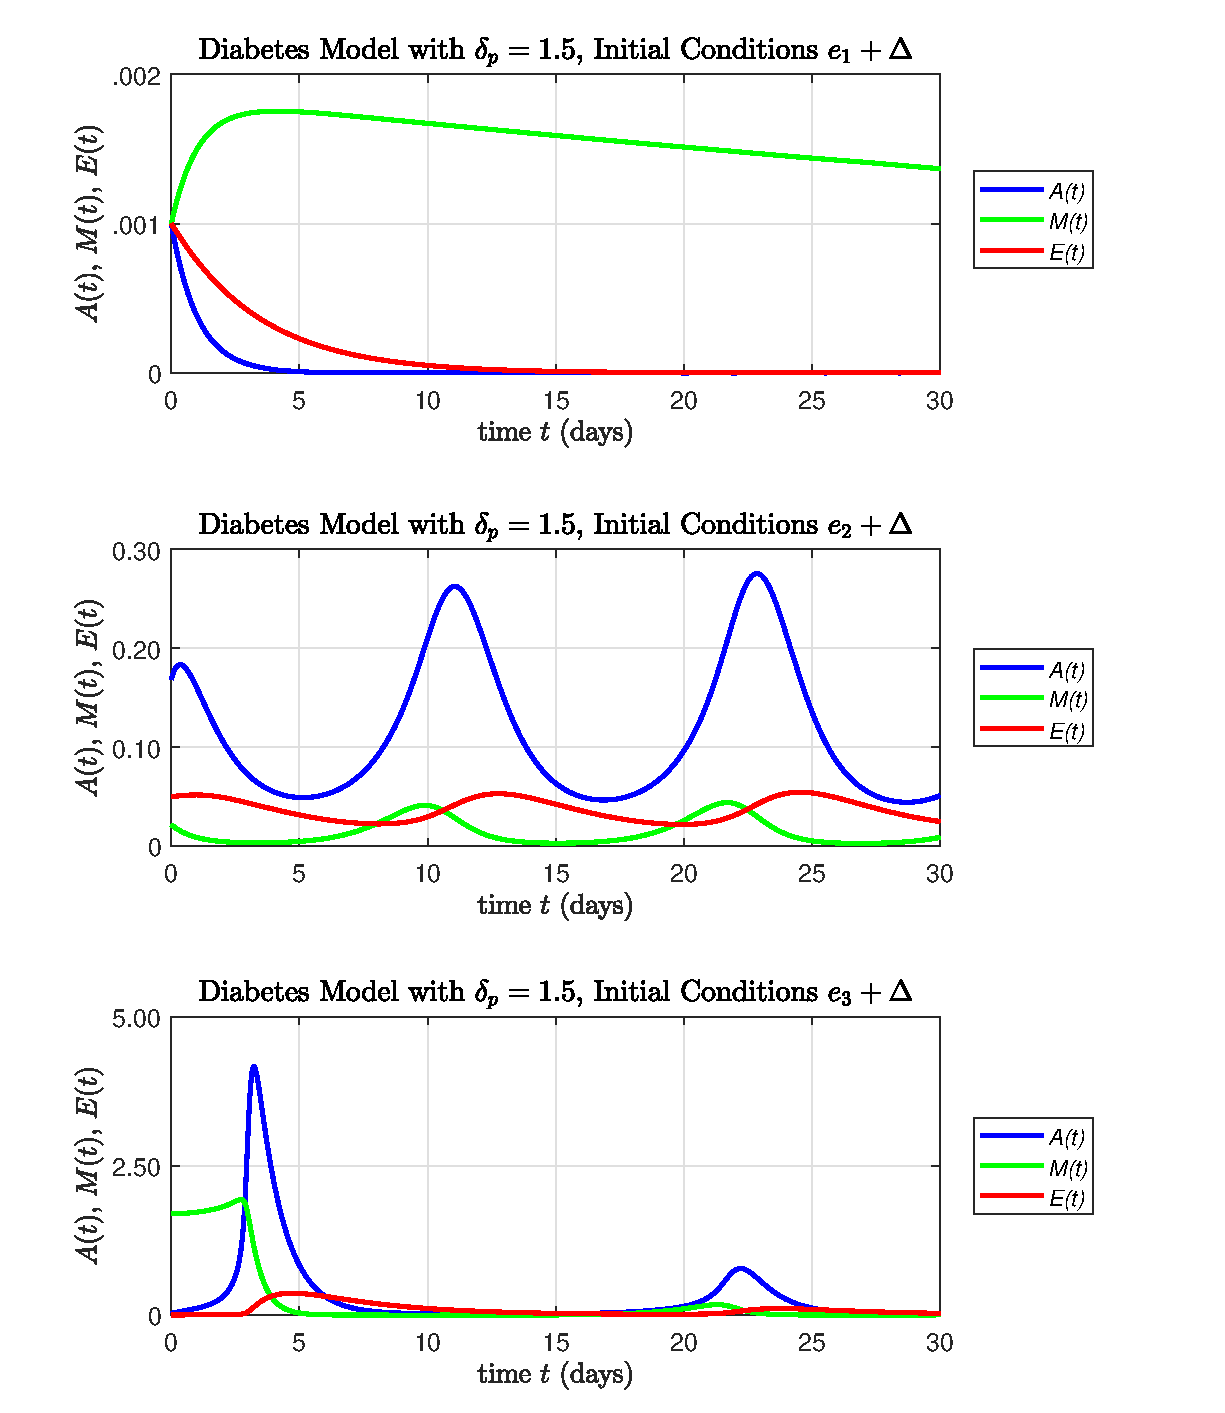
\includegraphics[width=16cm]{f3_3.eps}}
	\caption*{\textbf{Figure 3}}
\end{figure}

\end{document}





































